% ----- How it works -----

\subsection{How it works}

As said before, the local search algorithm takes an initial solution, and as long 
as a certain condition is not met, it looks at the neighbors of this initial solution 
and keeps the neighboring solution if it is better. Here is a rough overview of 
how all local search algorithms work:

\begin{enumerate}
    \item Finding an initial solution
    \item Look at a neighbor solution of the current one
    \begin{itemize}
        \item If the new solution is better than the old one, keep it as a solution
        \item Else, keep the old one as solution
    \end{itemize}
    \item As long as a certain stop condition has not been reached, repeat step 2
\end{enumerate}

First, in our case, finding the initial solution is done by taking the highest 
degree vertex, then its highest degree neighbor. These two vertices form a 
clique which will be improved to form a maximal clique as shown below:

\begin{minipage}{\linewidth}
    \textbf{Step 0:} \newline
    
    \begin{minipage}{0.4\textwidth}
        \begin{figure}[H]
            \centering
            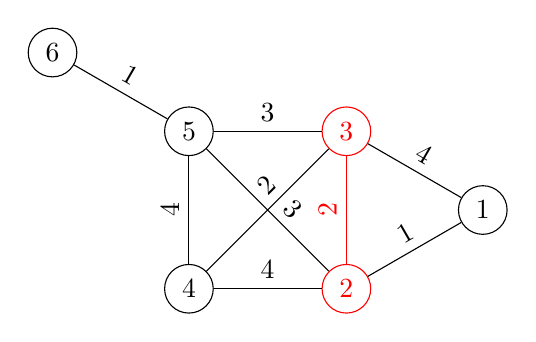
\begin{tikzpicture}[node distance=2cm]
                \node[circle, draw] (1) {1};
                \node[circle, draw, red] (2) at ([shift=(210:2)] 1) {2};
                \node[circle, draw] (4) [left of=2] {4};
                \node[circle, draw] (5) [above of=4] {5};
                \node[circle, draw, red] (3) [above of=2] {3};
                \node[circle, draw] (6) at ([shift=(150:2)] 5) {6};

                \draw (1) -- (2) node[midway, above, sloped] {1};
                \draw (1) -- (3) node[midway, above, sloped] {4};
                \draw (2) -- (4) node[midway, above, sloped] {4};
                \draw[red] (2) -- (3) node[midway, above, sloped] {2};
                \draw (4) -- (5) node[midway, above, sloped] {4};
                \draw (5) -- (3) node[midway, above, sloped] {3};
                \draw (5) -- (6) node[midway, above, sloped] {1};
                \draw (3) -- (4) node[midway, above right, sloped] {2};
                \draw (2) -- (5) node[midway, above right, sloped] {3};
            \end{tikzpicture}
            \caption{Graph illustration for the local search algorithm at step 0}
            \label{fig:local-search-mewc-init-0}
        \end{figure}
    \end{minipage}
    \begin{minipage}{0.6\textwidth}
        The first vertex to be taken will be $2$, of degree $4$. Among its neighbors 
        $\{1, 3, 4, 5\}$, the highest degree vertex is $4$ ($d(3) = 4$) so we form 
        a clique with the vertices $\{2, 3\}$.
    \end{minipage}
\end{minipage}

\vspace{1\baselineskip}

\begin{minipage}{\linewidth}
    \textbf{Step 1:} \newline
    
    \begin{minipage}{0.4\textwidth}
        \begin{figure}[H]
            \centering
            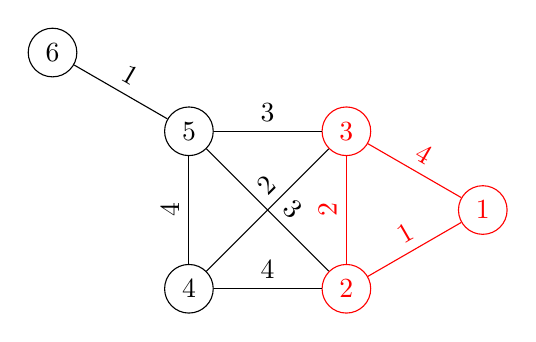
\begin{tikzpicture}[node distance=2cm]
                \node[circle, draw, red] (1) {1};
                \node[circle, draw, red] (2) at ([shift=(210:2)] 1) {2};
                \node[circle, draw] (4) [left of=2] {4};
                \node[circle, draw] (5) [above of=4] {5};
                \node[circle, draw, red] (3) [above of=2] {3};
                \node[circle, draw] (6) at ([shift=(150:2)] 5) {6};

                \draw[red] (1) -- (2) node[midway, above, sloped] {1};
                \draw[red] (1) -- (3) node[midway, above, sloped] {4};
                \draw (2) -- (4) node[midway, above, sloped] {4};
                \draw[red] (2) -- (3) node[midway, above, sloped] {2};
                \draw (4) -- (5) node[midway, above, sloped] {4};
                \draw (5) -- (3) node[midway, above, sloped] {3};
                \draw (5) -- (6) node[midway, above, sloped] {1};
                \draw (3) -- (4) node[midway, above right, sloped] {2};
                \draw (2) -- (5) node[midway, above right, sloped] {3};
            \end{tikzpicture}
            \caption{Graph illustration for the local search algorithm at step 1}
            \label{fig:local-search-mewc-init-1}
        \end{figure}
    \end{minipage}
    \begin{minipage}{0.6\textwidth}
        We can assume that the first vertex looked at to find a maximal clique will 
        be $1$, and as it is the neighbor of both $2$ and $3$ (all the vertices of 
        the current clique), we add it to the clique. We now look for common 
        neighbors of the three vertices of the clique: we find none, so the 
        clique $\{1, 2, 3\}$ forms a maximal clique: this is our initial solution 
        and its weight is $w(C_{init}) = 1+2+4 = 7$.
    \end{minipage}
\end{minipage}

\bigskip

We now have an initial solution. The objective will be to look at its neighbors to 
find a better solution (that is a maximal clique with a higher weight). This is done 
by deleting a vertex in our current solution. With one less vertex, the clique may 
not be maximal anymore, so we will try to make it maximal. If the weight of the new 
clique is greater than the old one, then we keep this new clique as the current 
solution. Otherwise, we keep the old one and try to improve it by removing another 
vertex. To choose which vertex to remove, we choose the one that adds the least 
weight to the clique. This will increase the chances of finding a better solution.

\begin{minipage}{\linewidth}
    \textbf{Step 2:} \newline
    
    \begin{minipage}{0.4\textwidth}
        \begin{figure}[H]
            \centering
            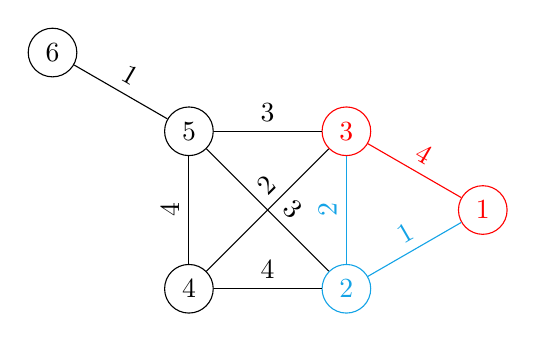
\begin{tikzpicture}[node distance=2cm]
                \node[circle, draw, red] (1) {1};
                \node[circle, draw, Cerulean] (2) at ([shift=(210:2)] 1) {2};
                \node[circle, draw] (4) [left of=2] {4};
                \node[circle, draw] (5) [above of=4] {5};
                \node[circle, draw, red] (3) [above of=2] {3};
                \node[circle, draw] (6) at ([shift=(150:2)] 5) {6};

                \draw[Cerulean] (1) -- (2) node[midway, above, sloped] {1};
                \draw[red] (1) -- (3) node[midway, above, sloped] {4};
                \draw (2) -- (4) node[midway, above, sloped] {4};
                \draw[Cerulean] (2) -- (3) node[midway, above, sloped] {2};
                \draw (4) -- (5) node[midway, above, sloped] {4};
                \draw (5) -- (3) node[midway, above, sloped] {3};
                \draw (5) -- (6) node[midway, above, sloped] {1};
                \draw (3) -- (4) node[midway, above right, sloped] {2};
                \draw (2) -- (5) node[midway, above right, sloped] {3};
            \end{tikzpicture}
            \caption{Graph illustration for the local search algorithm at step 2}
            \label{fig:local-search-mewc-neighbour-2}
        \end{figure}
    \end{minipage}
    \begin{minipage}{0.6\textwidth}
        Among the three vertices of the current solution, the $2$ is the one which 
        adds the least weight (if we remove it, we reduce the weight of the clique 
        by $2+1=3$). We obtain then a clique made up of the vertices $\{1, 3\}$. 
        Now, these two vertices have no neighbor in common, so this clique is 
        maximal and of weight $w(C_1) = 4$. As $w(C_1) = 4 < w(C_{init}) = 7$, we 
        do not keep this solution.
    \end{minipage}
\end{minipage}

\vspace{1\baselineskip}

\begin{minipage}{\linewidth}
    \textbf{Step 3:} \newline
    
    \begin{minipage}{0.4\textwidth}
        \begin{figure}[H]
            \centering
            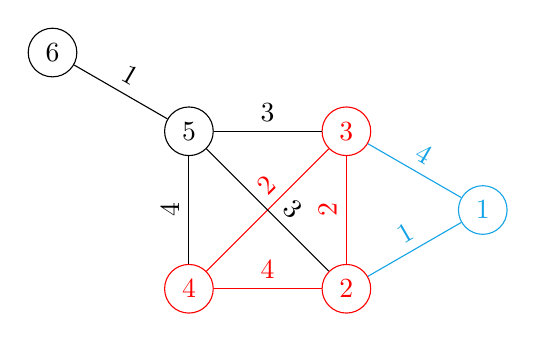
\begin{tikzpicture}[node distance=2cm]
                \node[circle, draw, Cerulean] (1) {1};
                \node[circle, draw, red] (2) at ([shift=(210:2)] 1) {2};
                \node[circle, draw, red] (4) [left of=2] {4};
                \node[circle, draw] (5) [above of=4] {5};
                \node[circle, draw, red] (3) [above of=2] {3};
                \node[circle, draw] (6) at ([shift=(150:2)] 5) {6};

                \draw[Cerulean] (1) -- (2) node[midway, above, sloped] {1};
                \draw[Cerulean] (1) -- (3) node[midway, above, sloped] {4};
                \draw[red] (2) -- (4) node[midway, above, sloped] {4};
                \draw[red] (2) -- (3) node[midway, above, sloped] {2};
                \draw (4) -- (5) node[midway, above, sloped] {4};
                \draw (5) -- (3) node[midway, above, sloped] {3};
                \draw (5) -- (6) node[midway, above, sloped] {1};
                \draw[red] (3) -- (4) node[midway, above right, sloped] {2};
                \draw (2) -- (5) node[midway, above right, sloped] {3};
            \end{tikzpicture}
            \caption{Graph illustration for the local search algorithm at step 3}
            \label{fig:local-search-mewc-neighbour-3}
        \end{figure}
    \end{minipage}
    \begin{minipage}{0.6\textwidth}
        The second vertex of minimum weight is $1$. If we remove it, we observe that 
        the vertex $4$ is adjacent to the two remaining vertices in the clique 
        ($\{2, 3\}$). So we add it to our solution, and we obtain the clique 
        $C_2 = \{2, 3, 4\}$ with $w(C_2) = 9$. Let's see if this clique is maximal or 
        if we can still improve it.
    \end{minipage}
\end{minipage}

\vspace{1\baselineskip}

\begin{minipage}{\linewidth}
    \textbf{Step 4:} \newline
    
    \begin{minipage}{0.4\textwidth}
        \begin{figure}[H]
            \centering
            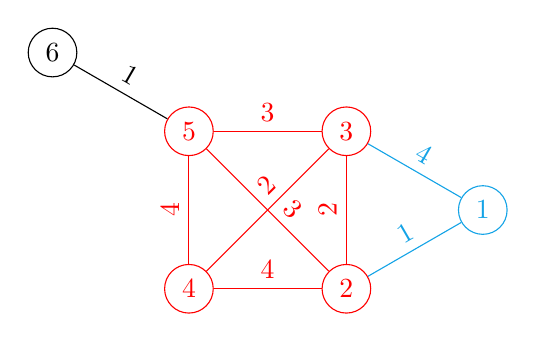
\begin{tikzpicture}[node distance=2cm]
                \node[circle, draw, Cerulean] (1) {1};
                \node[circle, draw, red] (2) at ([shift=(210:2)] 1) {2};
                \node[circle, draw, red] (4) [left of=2] {4};
                \node[circle, draw, red] (5) [above of=4] {5};
                \node[circle, draw, red] (3) [above of=2] {3};
                \node[circle, draw] (6) at ([shift=(150:2)] 5) {6};

                \draw[Cerulean] (1) -- (2) node[midway, above, sloped] {1};
                \draw[Cerulean] (1) -- (3) node[midway, above, sloped] {4};
                \draw[red] (2) -- (4) node[midway, above, sloped] {4};
                \draw[red] (2) -- (3) node[midway, above, sloped] {2};
                \draw[red] (4) -- (5) node[midway, above, sloped] {4};
                \draw[red] (5) -- (3) node[midway, above, sloped] {3};
                \draw (5) -- (6) node[midway, above, sloped] {1};
                \draw[red] (3) -- (4) node[midway, above right, sloped] {2};
                \draw[red] (2) -- (5) node[midway, above right, sloped] {3};
            \end{tikzpicture}
            \caption{Graph illustration for the local search algorithm at step 4}
            \label{fig:local-search-mewc-neighbour-4}
        \end{figure}
    \end{minipage}
    \begin{minipage}{0.6\textwidth}
        We can see that vertex $5$ is adjacent to all the vertices of $C_2$. We can 
        therefore add it to the clique: $C_2 = \{2, 3, 4, 5\}$ and $w(C_2) = 18$. We 
        notice that the vertices of the clique have no common neighbor, so we keep 
        $C_2$ as is. Furthermore, we then have $w(C_2) = 18$ greater than $w(C_{init}) = 7$. We 
        therefore take $C_2$ as the current solution.
    \end{minipage}
\end{minipage}

\bigskip

Now that we know how the solution is improved, all that remains is to see when the algorithm 
ends: what is the stop condition? A simple way to stop the algorithm is to define the stop 
condition as the moment when we have no more vertices to test, that is when we have removed 
all vertices one by one from the current solution without finding a better solution. Thus, 
we will have tested all the possibilities, and we will obtain a maximal clique which cannot 
be improved with this local search algorithm.